%%% DOCUMENT BEGIN

\documentclass{article}

\usepackage[utf8]{inputenc}

\usepackage{geometry}
\geometry{a4paper}

\usepackage{graphicx}
\usepackage{url}


%%% PACKAGES
\usepackage{booktabs} % for much better looking tables
\usepackage{array} % for better arrays (eg matrices) in maths
\usepackage{paralist} % very flexible & customisable lists (eg. enumerate/itemize, etc.)
\usepackage{verbatim} % adds environment for commenting out blocks of text & for better verbatim
\usepackage{subfig} % make it possible to include more than one captioned figure/table in a single float

%%% HEADERS & FOOTERS
\usepackage{fancyhdr} % This should be set AFTER setting up the page geometry
\pagestyle{fancy} % options: empty , plain , fancy
\renewcommand{\headrulewidth}{0pt} % customise the layout...
\lhead{}\chead{}\rhead{}
\lfoot{}\cfoot{\thepage}\rfoot{}

%%% SECTION TITLE APPEARANCE
\usepackage{sectsty}
\allsectionsfont{\sffamily\mdseries\upshape}

%%% ToC (table of contents) APPEARANCE
\usepackage[nottoc,notlof,notlot]{tocbibind} % Put the bibliography in the ToC
\usepackage[titles,subfigure]{tocloft} % Alter the style of the Table of Contents
\renewcommand{\cftsecfont}{\rmfamily\mdseries\upshape}
\renewcommand{\cftsecpagefont}{\rmfamily\mdseries\upshape} % No bold!


%%% END Article customizations

\usepackage[backend=biber, style=ieee]{biblatex}
\addbibresource{report.bib}
\usepackage{amssymb}
\usepackage{longtable}
\usepackage{ifthen}
\usepackage{pgfplots}
\pgfplotsset{compat=1.4}
%\usepackage{caption}
%\usepackage{subcaption}


%%%%%%%%%%%%%%%%%%%%%%%%%
%%%          Fill in the title details                      %%%

\def \thetitle {INF-3200 Distributed Systems}
\def \thesubtitle {Assignment 2 - P2P}
\def \theauthor {Camilla Stormoen \& Sigurd Thomassen}
\def \pagecount {5}

%%%%%%%%%%%%%%%%%%%%%%%%%

%\pagestyle{fancy}
\pagestyle{fancyplain} % options: empty , plain , fancy
\renewcommand{\headrulewidth}{1pt} % customise the layout...
\renewcommand{\footrulewidth}{0pt}
\lhead{\fancyplain{}{\thetitle{} -- \thesubtitle{}}}\chead{}\rhead{\fancyplain{}{\theauthor{}}}
\lfoot{}\cfoot{Page {\thepage} of \pagecount}\rfoot{}

\begin{document}

%%% TITLE PAGE

\begin{titlepage}
\begin{center}



\textsc{\\[3.5cm] \huge University of Tromsø}\\[1.5cm]

\textsc{\LARGE \thetitle}\\[0.5cm]

\textsc{\Large \thesubtitle}\\[1.5cm]

\LARGE{\theauthor} \\[0.5cm] \large{Department of Computer Science}



\vfill
{\large \today}

\end{center}
\thispagestyle{empty}
\end{titlepage}

\newpage{}


%%% TABLE OF CONTENTS

%\tableofcontents


\newpage{}

%%% DOCUMENT BODY

%%% Set counter to 1
\setcounter{page}{1}

\section{Introduction}

This report describes the implementation of a peer-to-peer network with dynamic join, and remove. It also discusses the performance and issues revolving the implementation of such a system.

\section{Technical Background}

\subsection{Peer-to-peer network} 
A peer-to-peer network is a distributed application that partitions tasks or work between peers. Peers are both clients and servers of resources and can be unstructured networks or structured networks. \cite{wiki:p2p}

\begin{figure}[h]
\begin{center}
%\fbox{
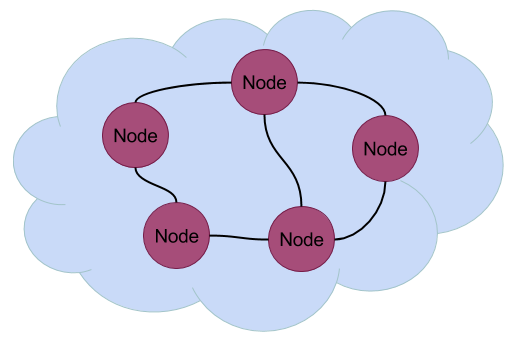
\includegraphics[scale=.6]
{p2p.png}
\end{center}
\caption{Peer-to-peer network }\label{fig:p2p}
\end{figure}

\subsection{Unstructured network}
Unstructured peer-to-peer networks are formed by nodes that randomly connect to each other. Because of the role of all nodes in the network is the same, unstructured networks are highly robust in the face of rates of “churn”. A churn is when large numbers of nodes are frequently joining and leaving the network. \cite{wiki:un}


\section{Design}
The distributed system implemented, is built upon the independence of each node. In a way where each node does not depend on a superior node managing it. It is a peer-to-peer network of nodes. Each node is an individual server running on a unique address.

\subsection{Initialization}
The initialization of the node is done by attempting to initiate a node on an address given when the first node is started. If the address is free, the node-server is started. If not, the node has to attempt a different port on the same ip, and do this until it finds a free port.
When the server is created, the node updates its neighbours, which in the first case will be itself. How the neighbours are updated will be explained in detail in a later section.
As well as being independent, each node runs on its own thread as well.
When more than one node is added to the network, a subprocess is started in the node which is told to add more nodes. These subprocesses will start their own nodes on their own threads. And each of them will update their connections, so that they all form a ring structure.


\begin{figure}[h]
\begin{center}
%\fbox{
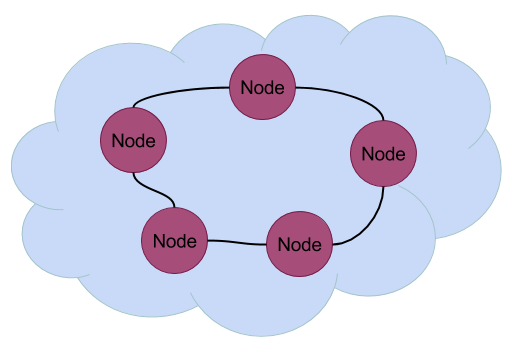
\includegraphics[scale=.6]
{our_p2p.png}
\end{center}
\caption{Peer-to-peer network with ring-structure}\label{fig:our_p2p}
\end{figure}

\subsection{Finding a free ip}
When the node is about to initialize, it needs a free address. This address is found by using a shell script looking for available nodes on the physical cluster. This script is run as a subprocess, and the result is directly used in the assignment of the ip. The default port used is port 8088, and if this is not free, the node will keep incrementing this until it finds a free one. This again makes the system support more nodes than the physical cluster has, as several nodes can be run on the same cluster node, but on different ports.

\subsection{Add node}
When a node is added, the \emph{main node} which is the one getting the call to add a node, will initiate a subprocess with the right parameters to invoke a new thread running the same program, but on a different address. This new node is added as the successor of the node it came from. And if it is the first node to be added, it will become the predecessor of the \emph{main node}. All subsequent nodes added, will start out as the successor of the \emph{main node}, but will be rearranged as more nodes are added.

\subsection{Neighbours}
When the new node is setting up, it will set its neighbours correctly, and it will call the neighbour nodes and tell them to update their connections as well. As they now need to reference this new node as a neighbour. These updates are done by using http requests to call the other nodes. And when a node get a specific request, they have to obey. An example would be to update the successor or predecessor. Then it will read the message from the caller, and use the address in the message to update either the successor or predecessor. As this is sent to both neighbours of a node, it will keep the ring structure intact, and no node will be left out of the ring.

\subsection{Shutdown nodes}
When a node receives a shutdown request, it will unlink itself from the ring structure. This is done by updating its neighbours to link to each other, around the current node. And then it will shut down the server it is running on, after it has returned confirmation to the caller that it is shutting down.


\section{Implementation}
The program is written in the programming language Python, and it is tested as a distributed system on a cluster, using up to X nodes. The performance evaluation of the system has been done by measuring the churn the system can handle.


\section{Discussion}
The program is built as a simple peer-to-peer system where the nodes are implemented as a ring-like structure where each node will contain a successor and a predecessor. Implementing this structured peer-to-peer system makes it easy to add a new node or to shut a node down.

It is a simple implementation, and it is quite naive. It does not support multiple joins at the same time, as it does not have locks implemented. However if the wait between each join is long enough, it might handle multiple joins from more than one client, as the timeout will now give leeway for the server to handle it.

When shutting down nodes, there are some connections that miss. This is probably caused by some stray references to neighbours after updating the neighbours when nodes have left the ring.

\subsection{Evaluation}
The churn of the system is measured in how many joins and leaves the system can handle within a time-frame.

\begin{figure}[h]
%\begin{table}[]
\centering
\caption{Churn, measured in seconds}
\label{my-label}
\begin{tabular}{llll}
Number of nodes & Total time to add nodes & Total time to shut down nodes & Total time \\
50              & 25                               & 23                                     & 48                 
\end{tabular}
%\end{table}
\end{figure}
Figure 3 shows the time to add and shut down 50 nodes in the network. Measuring the churn of the system will give a churn for 1 minute as 57 nodes. This is calculated by the number of nodes divided by the time used to join and leave the network. To find the number of node in one minute, 60 seconds is divided by the number of seconds per node join and leave.

\begin{equation}
(50/48) = 1.041
\end{equation}
\begin{equation}
(60/1.041) = 57.63
\end{equation}

Churn for 1 minute is 57 nodes.

\subsection{Improvements}
As this is a simple solution that does not support concurrent adding of nodes or removing nodes from the network, one could have improved the network by using locks when adding or removing a node from the network.
An improvement would be when adding a node, the node itself, the neighbours and the new node should be locked so another node can’t add or delete the specific node that is the creator.
The same goes when shutting down a node. Then the node itself and its neighbours must be locked so for example a new node can’t be added to the node that is going to be removed from the network. If locks are implemented, the network can support concurrent adding of nodes and concurrent removing of nodes.

\section{Conclusion}
This report concludes the design and implementation of a simple distributed peer-to-peer network with dynamic join and remove. It also discusses the churn of the system, as well as describing the shortcommings, and pointing out improvements that can be implemented.


%%% BIBLOGRAPHY

\newpage{}

\printbibliography


\end{document}
